\icode{E-MD-CA-L2-261115-002}
如图所示，斜面\(ABC\)中\(AB\)段粗糙，\(BC\)段光滑。物块以\qty{10}{m/s}的初速度从\(A\)点沿斜面向上滑行，到达\(C\)点速度恰好为零。已知\(BC\)段的长度为\qty{2}{m}，物块上滑过程中，在\(AB\)段的加速度是\(BC\)段加速度的 \(1.5\) 倍，且物块在\(AB\)段和\(BC\)段运动的时间相等，\(g\) 取\qty{10}{m/s^2}，求：
\begin{enumerate}
	\item 斜面\(AB\)段的长度；
	\item 物块与斜面\(AB\)段间的动摩擦因数。
\end{enumerate}

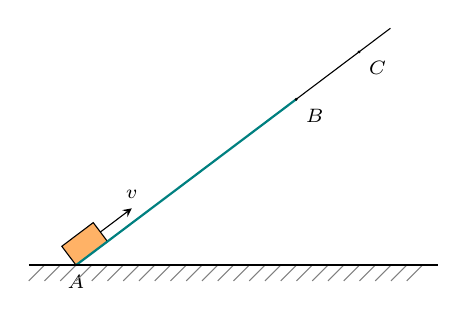
\begin{tikzpicture}[>=stealth,font=\scriptsize]
	\begin{scope}[rotate=37]
		\draw[fill=orange!60] (0,0) rectangle(.5,.3);
		\draw[->] (.5,.15)--(1,.15)node[above]{\(v\)};
		\draw[thick,teal] (0,0)--(3.5,0)coordinate(b);
		\draw[thin] (3.5,0)--(5,0);
		\coordinate (c) at(4.5,0);
	\end{scope}
	\fill (b)node[below right]{\(B\)} circle(.02) (c)node[below right]{\(C\)} circle(.02);
	\node at(0,0)[below]{\(A\)};
	\foreach \x in {-.6,-.4,...,4.4}
		\draw[gray] (\x,-.2)--++(.2,.2);
	\draw[thick] (-.6,0)--(4.6,0);
\end{tikzpicture}
\begin{answer}
    （1）\qty{7}{m}（2）\(\mu = \frac{\sqrt{21}}{21} \)
\end{answer}